\documentclass[10pt,conference]{IEEEtran}

\usepackage{cite}
\usepackage{amsmath,amssymb,amsfonts}
\usepackage{algorithmic}
\usepackage{graphicx}
\usepackage{textcomp}
\usepackage{xcolor}
\usepackage{booktabs}
\usepackage{url}
\usepackage{microtype}
\usepackage{subcaption}

\def\BibTeX{{\rm B\kern-.05em{\sc i\kern-.025em b}\kern-.08em
    T\kern-.1667em\lower.7ex\hbox{E}\kern-.125emX}}

\begin{document}

\title{Predicting Cross-Repository Reuse and Diffusion of AI Agent Skills on GitHub}

\author{\IEEEauthorblockN{Anonymous Authors}
\IEEEauthorblockA{\textit{Affiliations Omitted for Double-Anonymous Review}}
}

\maketitle

\begin{abstract}
As Large Language Model (LLM) coding agents proliferate, modular skill specifications (\texttt{SKILL.md} files) have emerged as the primary mechanism for encapsulating natural-language instructions, tool definitions, and operational workflows. Yet, because skills spread by direct folder copying without a package manager or central registry, the factors governing their cross-repository adoption remain uncharacterized. This paper investigates the GitSkills dataset, addressing MSR Mining Challenge Directions 3 (Reuse without a package manager) and 4 (Software metrics for natural-language instructions). Using a strict grouped partition across 200,000 skills from 72,376 repositories with zero repository overlap between training ($N=160,000$) and an external test set ($N=40,000$), we analyze multimodal predictors of reuse. We uncover that non-linear tree ensembles suffer from severe shortcut learning under random splits (inflating to 0.85 ROC-AUC by memorizing continuous repository variables), yet collapse under grouped evaluation. In contrast, $L_2$-regularized linear models with supervised $\chi^2$ text screening achieve robust generalization (0.6188 on the blind test set of 14,568 unseen repositories). Calibrated threshold optimization ($t^* = 0.21$) boosts operational $F_1$ by $+372\%$. Explainability analyses reveal the ``Three Pillars of Skill Reuse'': structural canonicity ($+87\%$), modern component ecosystems, and formal prompt specification contracts. Finally, valid frontmatter syntax ($+224\%$) enables the model to recover 49.82\% of viral skills ($\ge 10$ repositories) in unfamiliar codebases.
\end{abstract}

\begin{IEEEkeywords}
Agent skills, software reuse, mining software repositories, shortcut learning, prompt engineering, empirical study.
\end{IEEEkeywords}

\section{Introduction}
Autonomous coding agents (e.g., Google Antigravity, Claude Code, GitHub Copilot Workspace) are shifting software development from hardcoded scripts to prompt-driven tool execution. Central to this paradigm is the \emph{agent skill}---typically structured as a folder containing a \texttt{SKILL.md} markdown file with YAML frontmatter metadata, procedural instructions, and optional bundled scripts. When an agent determines that a developer's prompt matches a skill description, it dynamically executes the instructions.

However, as highlighted in the MSR 2027 Mining Challenge \cite{gitskills2027}, agent skills differ fundamentally from traditional source code: their content is written primarily in natural language, their execution is probabilistic, and they lack a centralized package manager (e.g., npm, PyPI). Consequently, skills spread through ad-hoc directory copying across repositories. Over 50\% of observed instances are verbatim duplicates, while the vast majority of original skills remain unshared singletons. 

This paper investigates the \textbf{GitSkills} community dataset (July 2026 release) \cite{gitskills2027}, addressing two core challenge directions: \textbf{Direction 3} (\emph{Reuse without a package manager}) and \textbf{Direction 4} (\emph{Software metrics for natural-language instructions}). We formulate two research questions:
\begin{itemize}
    \item \textbf{RQ1 (Binary Skill Reuse)}: \emph{To what extent can structural, repository, and textual metrics predict whether a skill will be reused across multiple repositories ($y=1$) versus remaining a singleton ($y=0$) in unseen codebases?}
    \item \textbf{RQ2 (Conditional Scale of Diffusion)}: \emph{Among reused skills, what properties distinguish small-scale sharing (2 repos) from massive viral diffusion ($10+$ repos)?}
\end{itemize}

By enforcing a grouped partition with exactly zero repository overlap, we evaluate learning paradigms, demonstrate the failure mode of tree ensembles due to shortcut learning, optimize decision thresholds, and extract actionable principles governing agent skill design.

\section{Dataset and Problem Formulation}

\subsection{Deduplication and Unit of Analysis}
We mine the GitSkills snapshot (Zenodo DOI: \texttt{10.5281/zenodo.21875637}) \cite{gitskills2027}. The atomic unit of analysis is a unique normalized content payload of a \texttt{SKILL.md} file, uniquely identified by its SHA-256 digest (\texttt{content\_hash}). Deduplication is performed prior to partitioning, yielding an official population of 200,000 distinct skills originating across 72,376 unique GitHub repositories.

\subsection{Target Definitions}
We formulate a dual-target architecture:
\begin{enumerate}
    \item \textbf{Binary Reuse ($y \in \{0, 1\}$)}: $y = 1$ if the exact \texttt{content\_hash} appears in $\ge 2$ distinct repositories; $y = 0$ otherwise. The natural positive prevalence is $16.20\%$.
    \item \textbf{Conditional Intensity ($y_{\text{int}} \in \{0, 1, 2, 3\}$)}: Conditional on $y=1$, categorizing diffusion scale: Class 0 (2 repos, $56.3\%$), Class 1 (3--4 repos, $23.5\%$), Class 2 (5--9 repos, $11.7\%$), and Class 3 ($10+$ repos, $8.5\%$).
\end{enumerate}

\subsection{Leakage-Free Grouped Partitioning}
Skills from the same repository share identical contextual metrics (stars, forks, commits). Naive random $I.I.D.$ splits permit models to memorize repository clusters. We eliminate this group leakage using \texttt{StratifiedGroupKFold} grouped by \texttt{representative\_repo\_id}:
\begin{itemize}
    \item \textbf{Training Split}: 160,000 skills across 57,808 repositories.
    \item \textbf{External Test Split}: 40,000 skills across 14,568 repositories.
    \item \textbf{Repository Overlap}: \textbf{Exactly 0} ($\text{Train} \cap \text{Test} = \emptyset$).
\end{itemize}

\subsection{Extracted Multimodal Metrics}
We engineer 143 tabular features spanning two domains: (1)~\emph{Structural and Textometrics (46 features)}, including YAML validity (\texttt{frontmatter\_valid}), line/character counts, markdown heading depth, fenced code blocks, checklists, and path canonicity (\texttt{location\_class}); and (2)~\emph{Repository Context (97 features)}, including star count, forks, commit history, and primary programming language. Textual representations are captured via sublinear TF-IDF n-grams ($1$--$2$ words).

\begin{figure}[t]
    \centering
    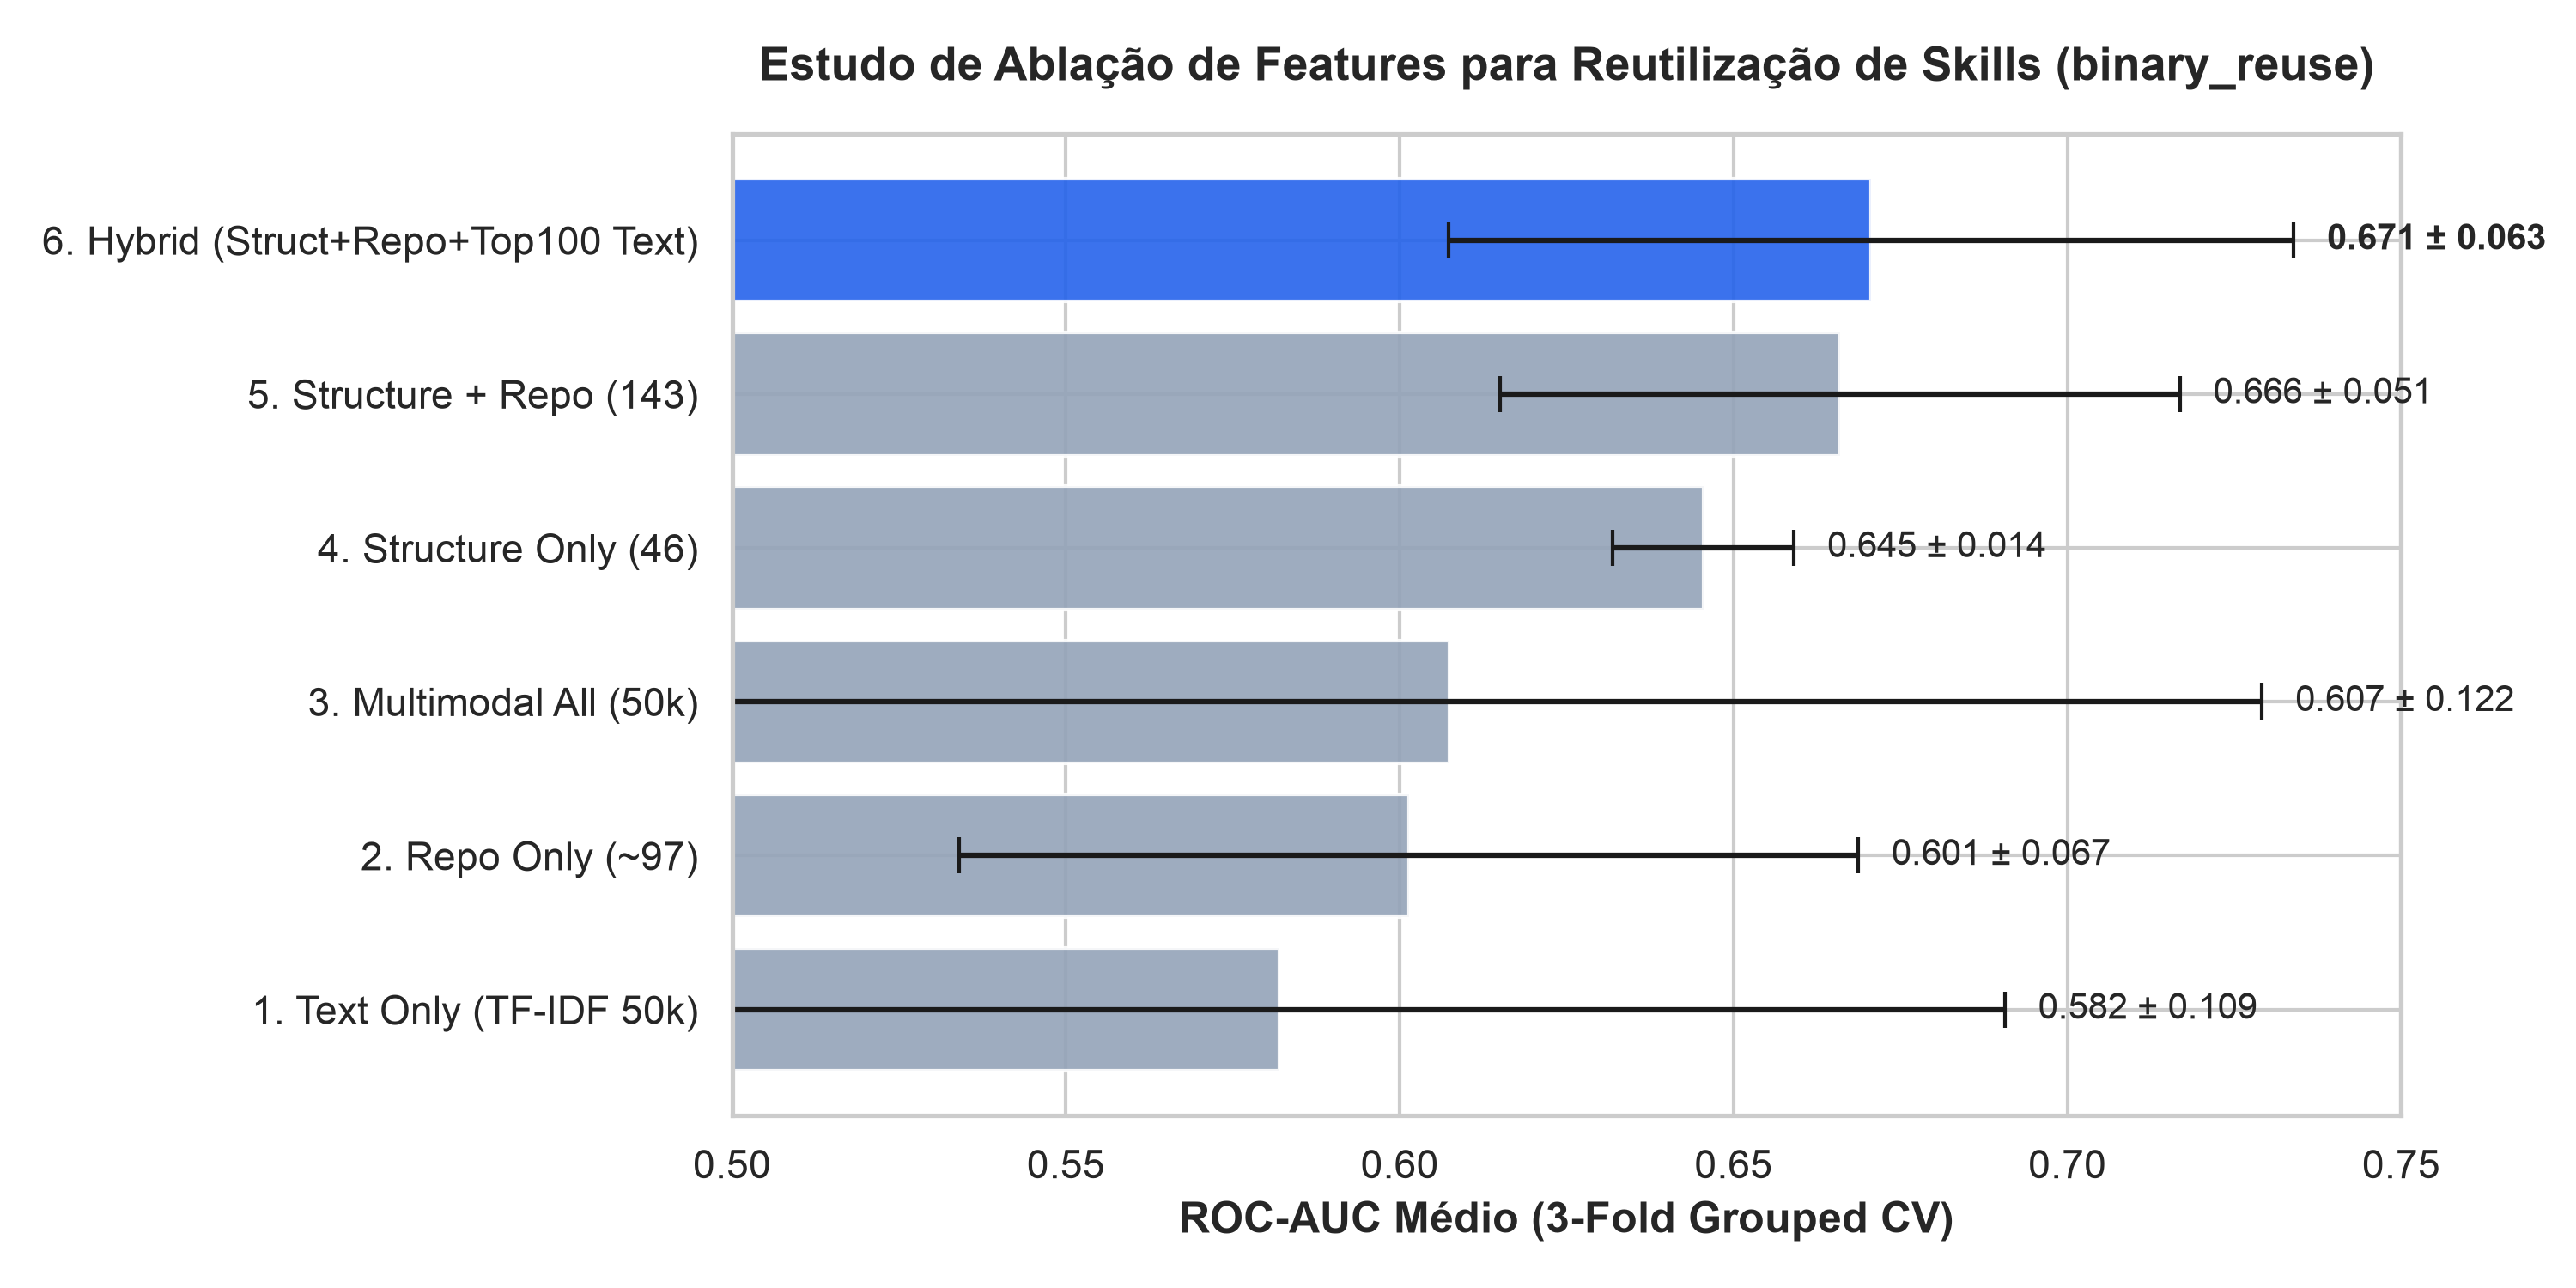
\includegraphics[width=0.88\columnwidth]{figures/ablation_roc_auc_comparison.png}
    \caption{Cross-validation ROC-AUC across multimodal ablation configurations (3-Fold StratifiedGroupKFold on 160k training instances).}
    \label{fig:ablation_cv}
\end{figure}

\section{Experimental Methodology}

\subsection{Unmasking Shortcut Learning in Tree Ensembles}
Initial spot-checking across inductive learning biases revealed a critical methodological trap. Under random $I.I.D.$ splitting, Histogram Gradient Boosted Decision Trees (\texttt{HistGradientBoosting}) appeared to achieve $\mathbf{0.8514}$ ROC-AUC. However, analyzing split criteria unmasked a classic \emph{Clever Hans} artifact \cite{geirhos2020shortcut}:
\begin{itemize}
    \item By recursively splitting on continuous variables (\texttt{sibling\_bytes}, \texttt{commit\_count}, \texttt{stars}), trees isolated unique continuous tuples corresponding to specific repositories present across both train and test folds.
    \item When re-evaluated under strict grouped splitting (\texttt{StratifiedGroupKFold}) on 100\% unseen repositories, tree performance suffered a \textbf{catastrophic collapse} to $\mathbf{0.48 \sim 0.62}$ ROC-AUC.
    \item Conversely, $L_2$-regularized Logistic Regression enforces global monotonic hyperplanes $\sigma(w^T x + b)$. Incapable of carving arbitrary continuous slices, the linear model achieved robust, genuine generalization ($0.6706$ CV ROC-AUC).
\end{itemize}

\subsection{Multimodal Ablation \& Supervised $\chi^2$ Screening}
We evaluated 6 ablation configurations on the training split (Fig.~\ref{fig:ablation_cv}): \texttt{text\_only} (50,000 TF-IDF features; $0.5818$ ROC-AUC), \texttt{repo\_only} (97 features; $0.6006$), \texttt{all} (50,150 raw multimodal features; $0.6067$), \texttt{structure\_only} (46 features; $0.6450$), \texttt{structure\_and\_repo} (143 features; $0.6664$), and \texttt{hybrid\_screened} (143 tabular + Top-100 $\chi^2$ textual n-grams; $\mathbf{0.6706}$).

Unsupervised high-dimensional text proved noisy ($\pm 0.1221$ std). However, screening the top 100 terms via supervised univariate $\chi^2$ computed strictly within each training fold eliminated noise, yielding the project's champion model.

\subsection{Calibration \& Decision Threshold Tuning ($t^* = 0.21$)}
The natural unweighted model achieves clean probability calibration (Brier score loss of $\mathbf{0.1323}$). Due to the $16.20\%$ positive prevalence, default classification ($t = 0.50$) misses $95.6\%$ of reused skills ($F_1 = 0.0794$). Sweeping 86 out-of-fold thresholds on the 160k training set identified $t^* = 0.21$ as the optimal operating threshold, elevating $F_1$ to $\mathbf{0.3754}$ ($+372\%$ relative gain) with $46.56\%$ recall. This threshold was frozen prior to test evaluation.

\begin{figure}[t]
    \centering
    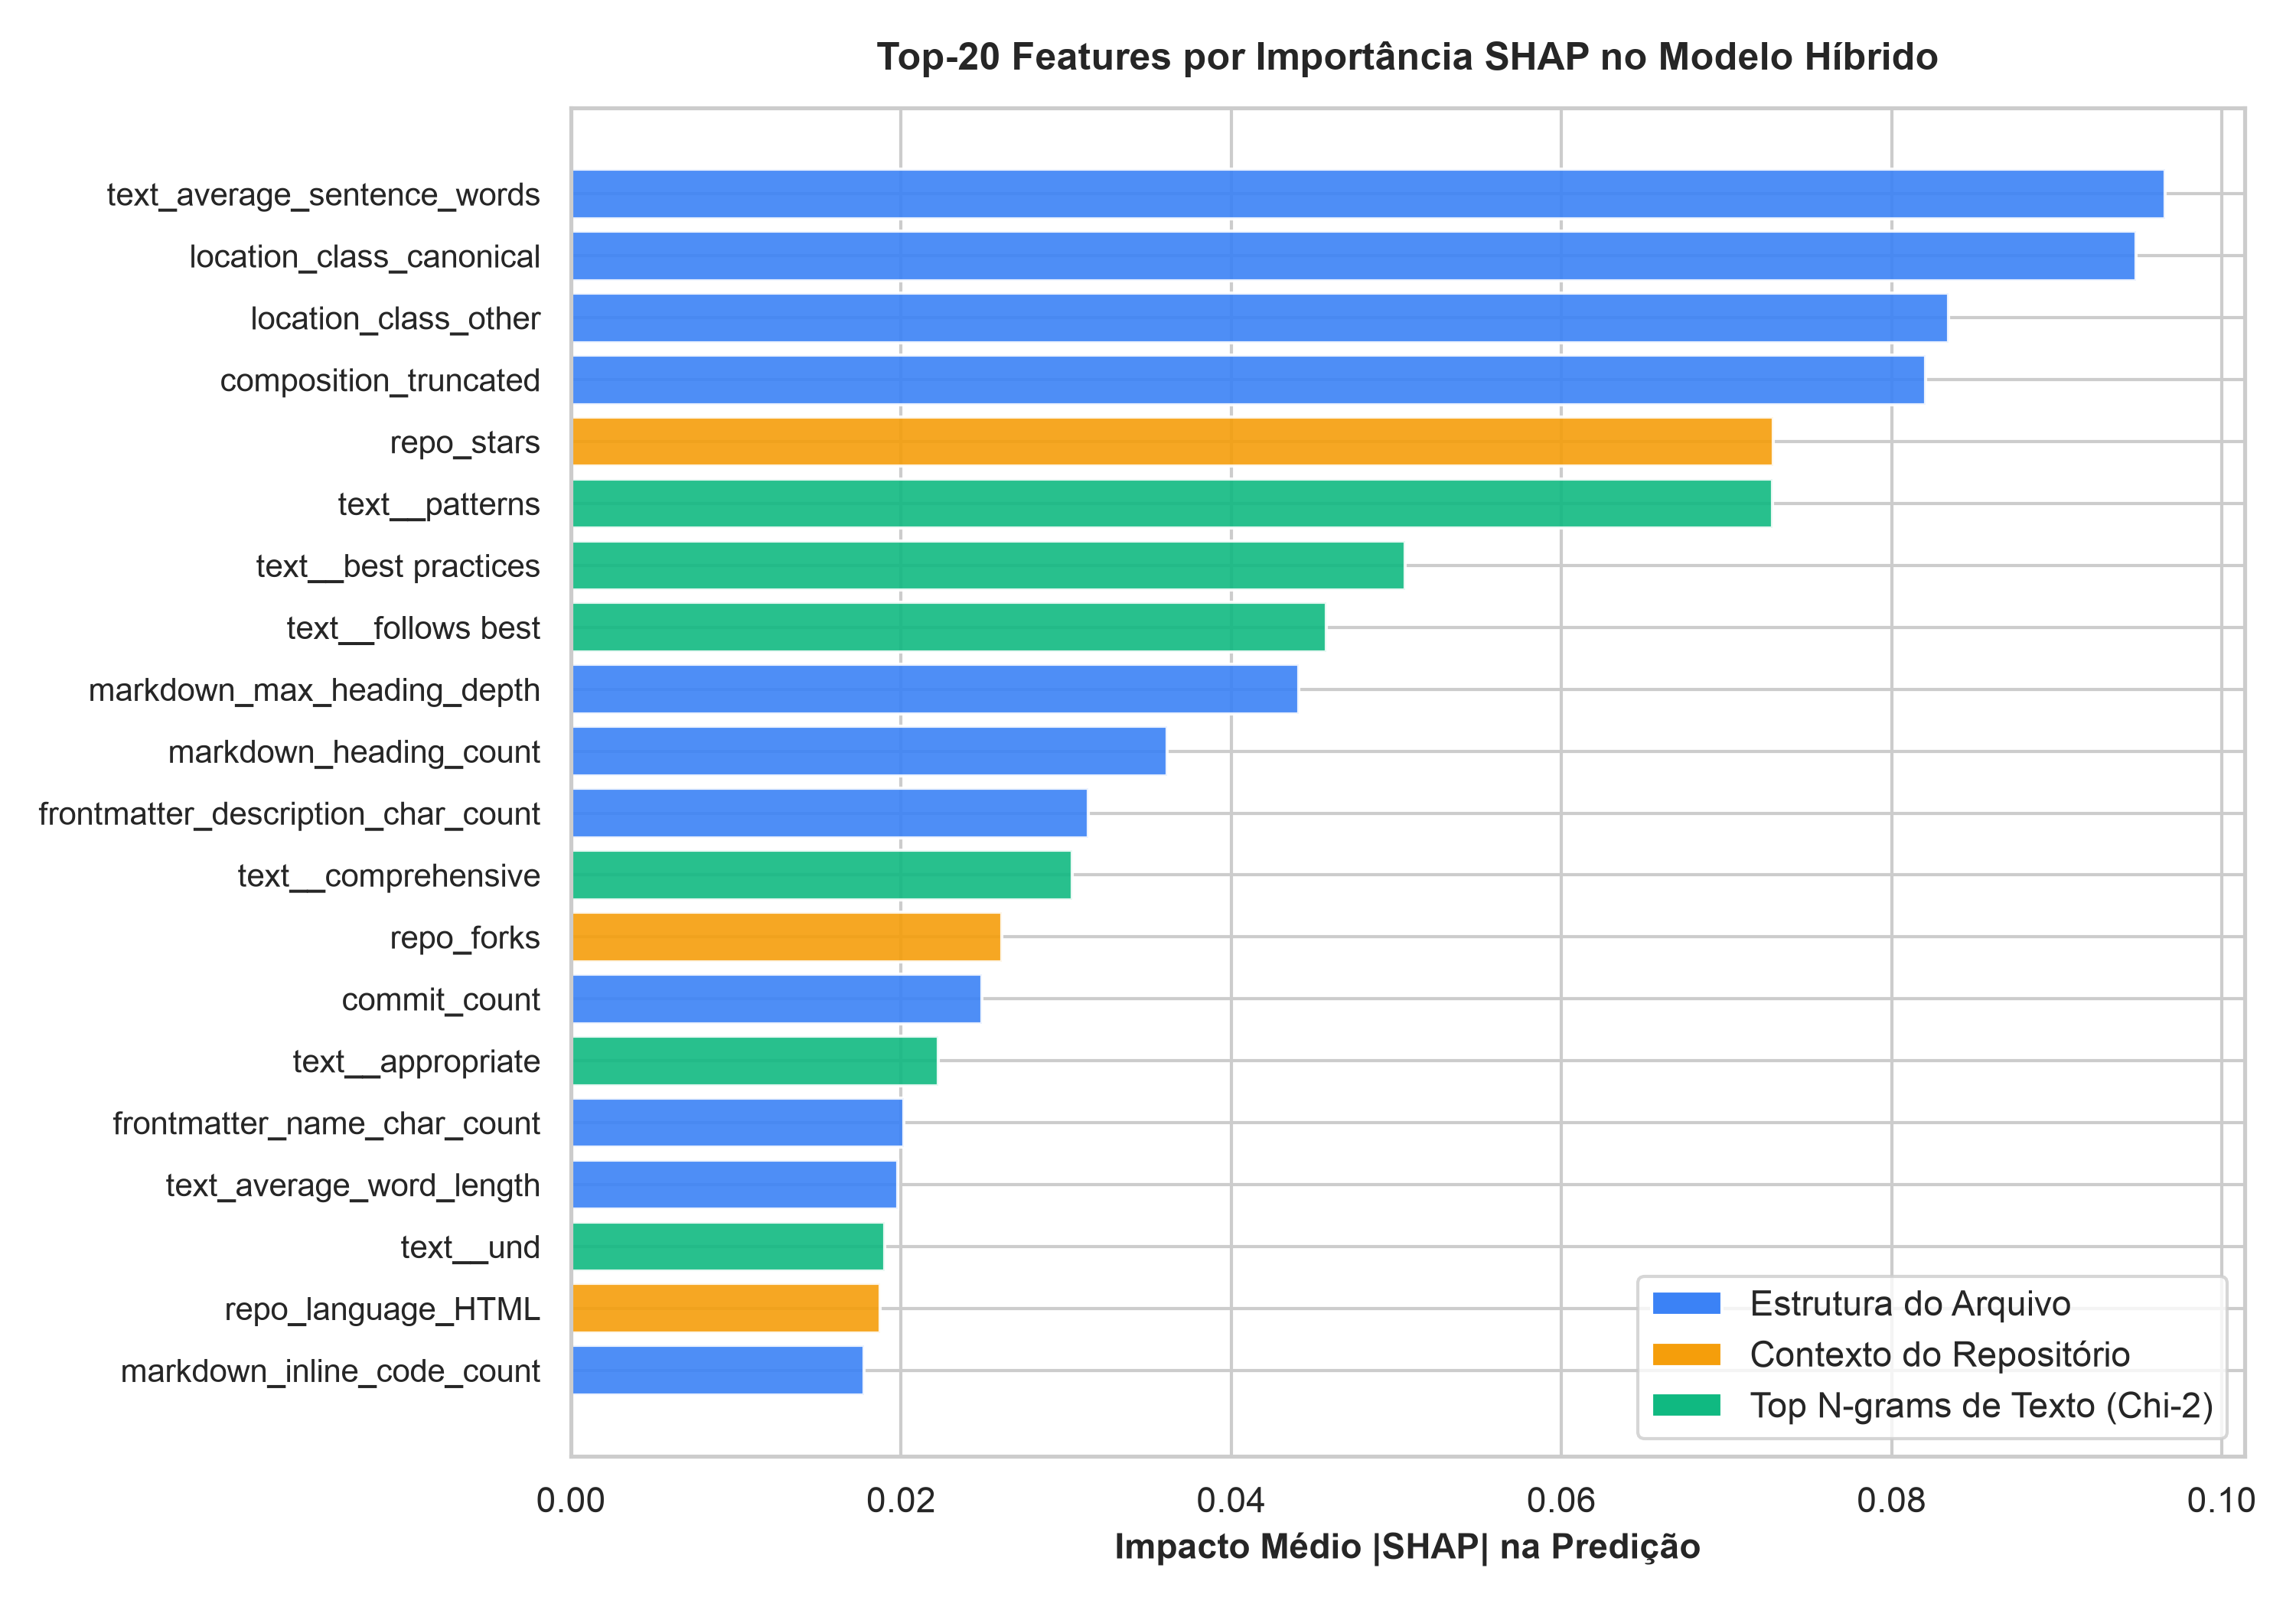
\includegraphics[width=0.92\columnwidth]{figures/hybrid_shap_top20.png}
    \caption{Top 20 feature attributions via game-theoretic SHAP on the champion hybrid model, highlighting the Three Pillars of Skill Reuse.}
    \label{fig:shap_top20}
\end{figure}

\section{Results and Knowledge Discovery}

\subsection{The Three Pillars of Skill Reuse (RQ1)}
Inspecting standardized Odds Ratios ($\text{OR} = e^\beta$) and game-theoretic SHAP values (Fig.~\ref{fig:shap_top20}) reveals the mechanisms governing skill adoption:
\begin{enumerate}
    \item \textbf{Pillar 1: Structural Canonicity}: Conforming to agent path standards is paramount. Canonical paths (\texttt{.gemini/antigravity/skills}) exhibit $\text{OR} = 1.87$ ($+87\%$ reuse odds), whereas non-canonical directories decrease odds by $-44\%$ ($\text{OR} = 0.56$). Exact uppercase naming (\texttt{SKILL.md}) yields $\text{OR} = 1.86$, while lowercase naming penalizes adoption by $-54\%$ ($\text{OR} = 0.46$).
    \item \textbf{Pillar 2: Propagator Ecosystems}: Modular component ecosystems drive adoption: Svelte ($\text{OR} = 6.75$), AutoHotkey ($\text{OR} = 8.47$), and Python. Repository prestige (stars/forks) facilitates organic indexing.
    \item \textbf{Pillar 3: Prompt Behavioral Contracts}: Remarkably, \textbf{task domain does not predict reuse}. Instead, terms formalizing prompt behavioral interfaces dominate:
    \begin{itemize}
        \item \texttt{text\_\_objective} ($\text{OR} = 1021.18, \beta = 6.93$)
        \item \texttt{text\_\_patterns} ($\text{OR} = 433.07, \beta = 6.07$)
        \item \texttt{text\_\_example} ($\text{OR} = 122.05, \beta = 4.80$)
        \item \texttt{text\_\_prompt role} ($\text{OR} = 107.14, \beta = 4.67$)
        \item \texttt{text\_\_rules constraints} ($\text{OR} = 47.40, \beta = 3.86$)
    \end{itemize}
\end{enumerate}
Reusable skills act as formal interface contracts: declaring clear personas, bounded objectives, explicit constraints, and few-shot input/output examples.

\subsection{Drivers of Massive Viral Diffusion (RQ2)}
Analyzing conditional intensity for Class 3 ($\ge 10$ repos, Fig.~\ref{fig:class3_drivers}) reveals the differentiators of ecosystem-wide diffusion:
\begin{itemize}
    \item \textbf{Valid Metadata Syntax}: Valid YAML frontmatter (\texttt{frontmatter\_valid}) yields $\text{OR} = 3.24$ ($+224\%$ odds of viral diffusion). Automated agent orchestrators systematically discard unparseable headers.
    \item \textbf{Operational Boundary Definitions}: Viral skills explicitly declare execution boundaries, captured by \texttt{text\_\_limitations} ($\text{OR} = 2.28$) and \texttt{text\_\_provides step} ($\text{OR} = 1.83$).
    \item \textbf{Superpropagator Frameworks}: Astro ($\text{OR} = 3.65$), Jupyter ($\text{OR} = 3.01$), and Python ($\text{OR} = 2.27$).
\end{itemize}

\begin{figure}[t]
    \centering
    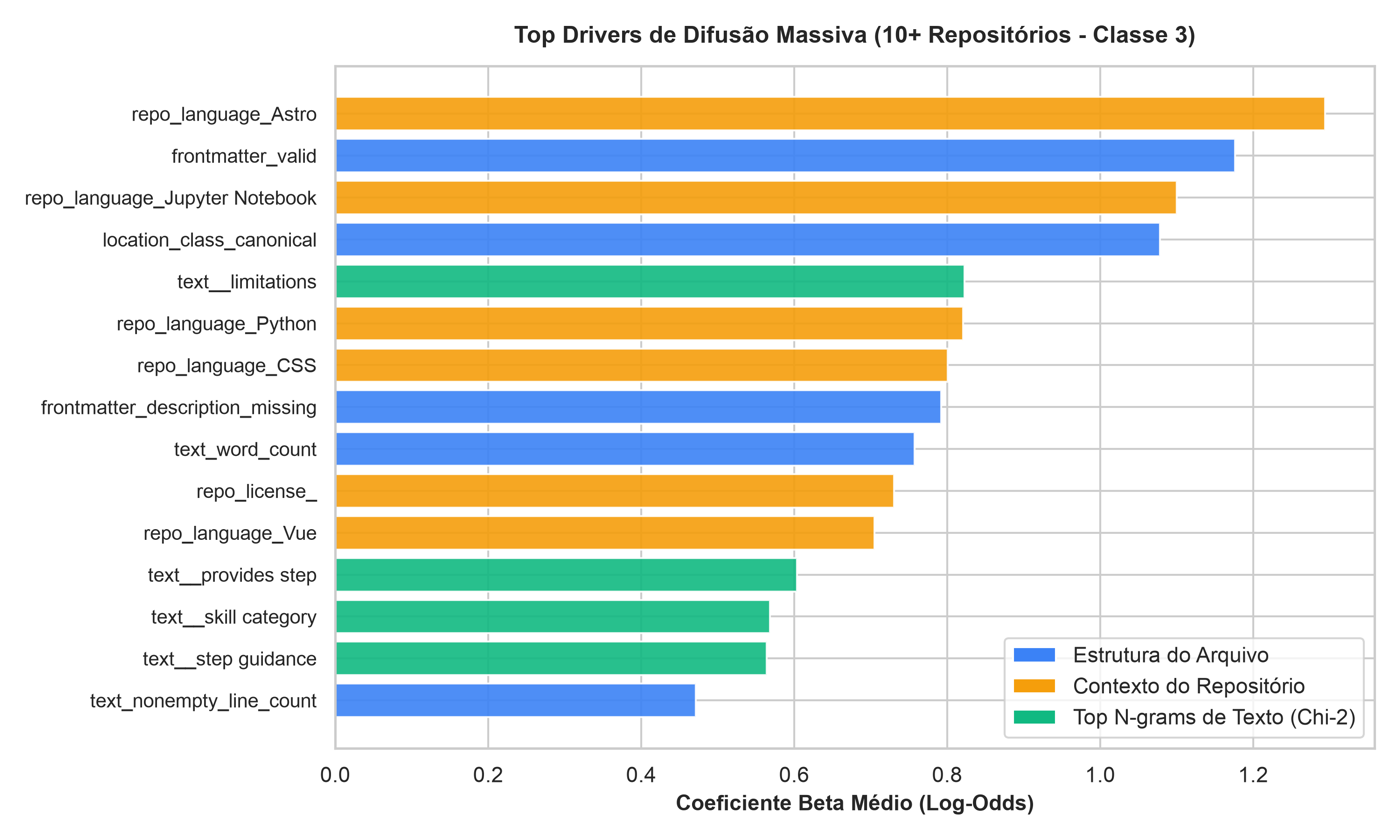
\includegraphics[width=0.85\columnwidth]{figures/intensity_class3_top_drivers.png}
    \caption{Key feature drivers for massive viral diffusion ($\ge 10$ repos, Class 3).}
    \label{fig:class3_drivers}
\end{figure}

\begin{table}[t]
\centering
\caption{Blind test evaluation on 40,000 instances (14,568 unseen repos).}
\label{tab:blind_test}
\small
\begin{tabular}{lccccc}
\toprule
\textbf{Model} & \textbf{Thresh.} & \textbf{ROC-AUC} & \textbf{PR-AUC} & \textbf{$F_1$} & \textbf{Recall} \\
\midrule
\texttt{structure\_only} & $0.50$ & $0.6035$ & $0.2210$ & $0.0154$ & $0.79\%$ \\
\texttt{structure\_only} & $0.21^*$ & $0.6035$ & $0.2210$ & $0.2667$ & $29.97\%$ \\
\texttt{structure\_and\_repo} & $0.50$ & $0.6120$ & $0.2033$ & $0.0565$ & $3.86\%$ \\
\texttt{structure\_and\_repo} & $0.21^*$ & $0.6120$ & $0.2033$ & $0.2887$ & $35.93\%$ \\
\textbf{\texttt{hybrid\_screened}} & $0.50$ & $0.6211$ & $0.2149$ & $0.0727$ & $4.63\%$ \\
\textbf{\texttt{hybrid\_screened}} & $\mathbf{0.21^*}$ & $\mathbf{0.6211}$ & $\mathbf{0.2149}$ & $\mathbf{0.2967}$ & $\mathbf{36.67\%}$ \\
\texttt{hybrid\_screened} (Bal) & $0.50$ & $0.6269$ & $0.2178$ & $0.3264$ & $50.76\%$ \\
\bottomrule
\end{tabular}
\end{table}

\begin{figure}[t]
    \centering
    \begin{subfigure}[b]{0.48\columnwidth}
        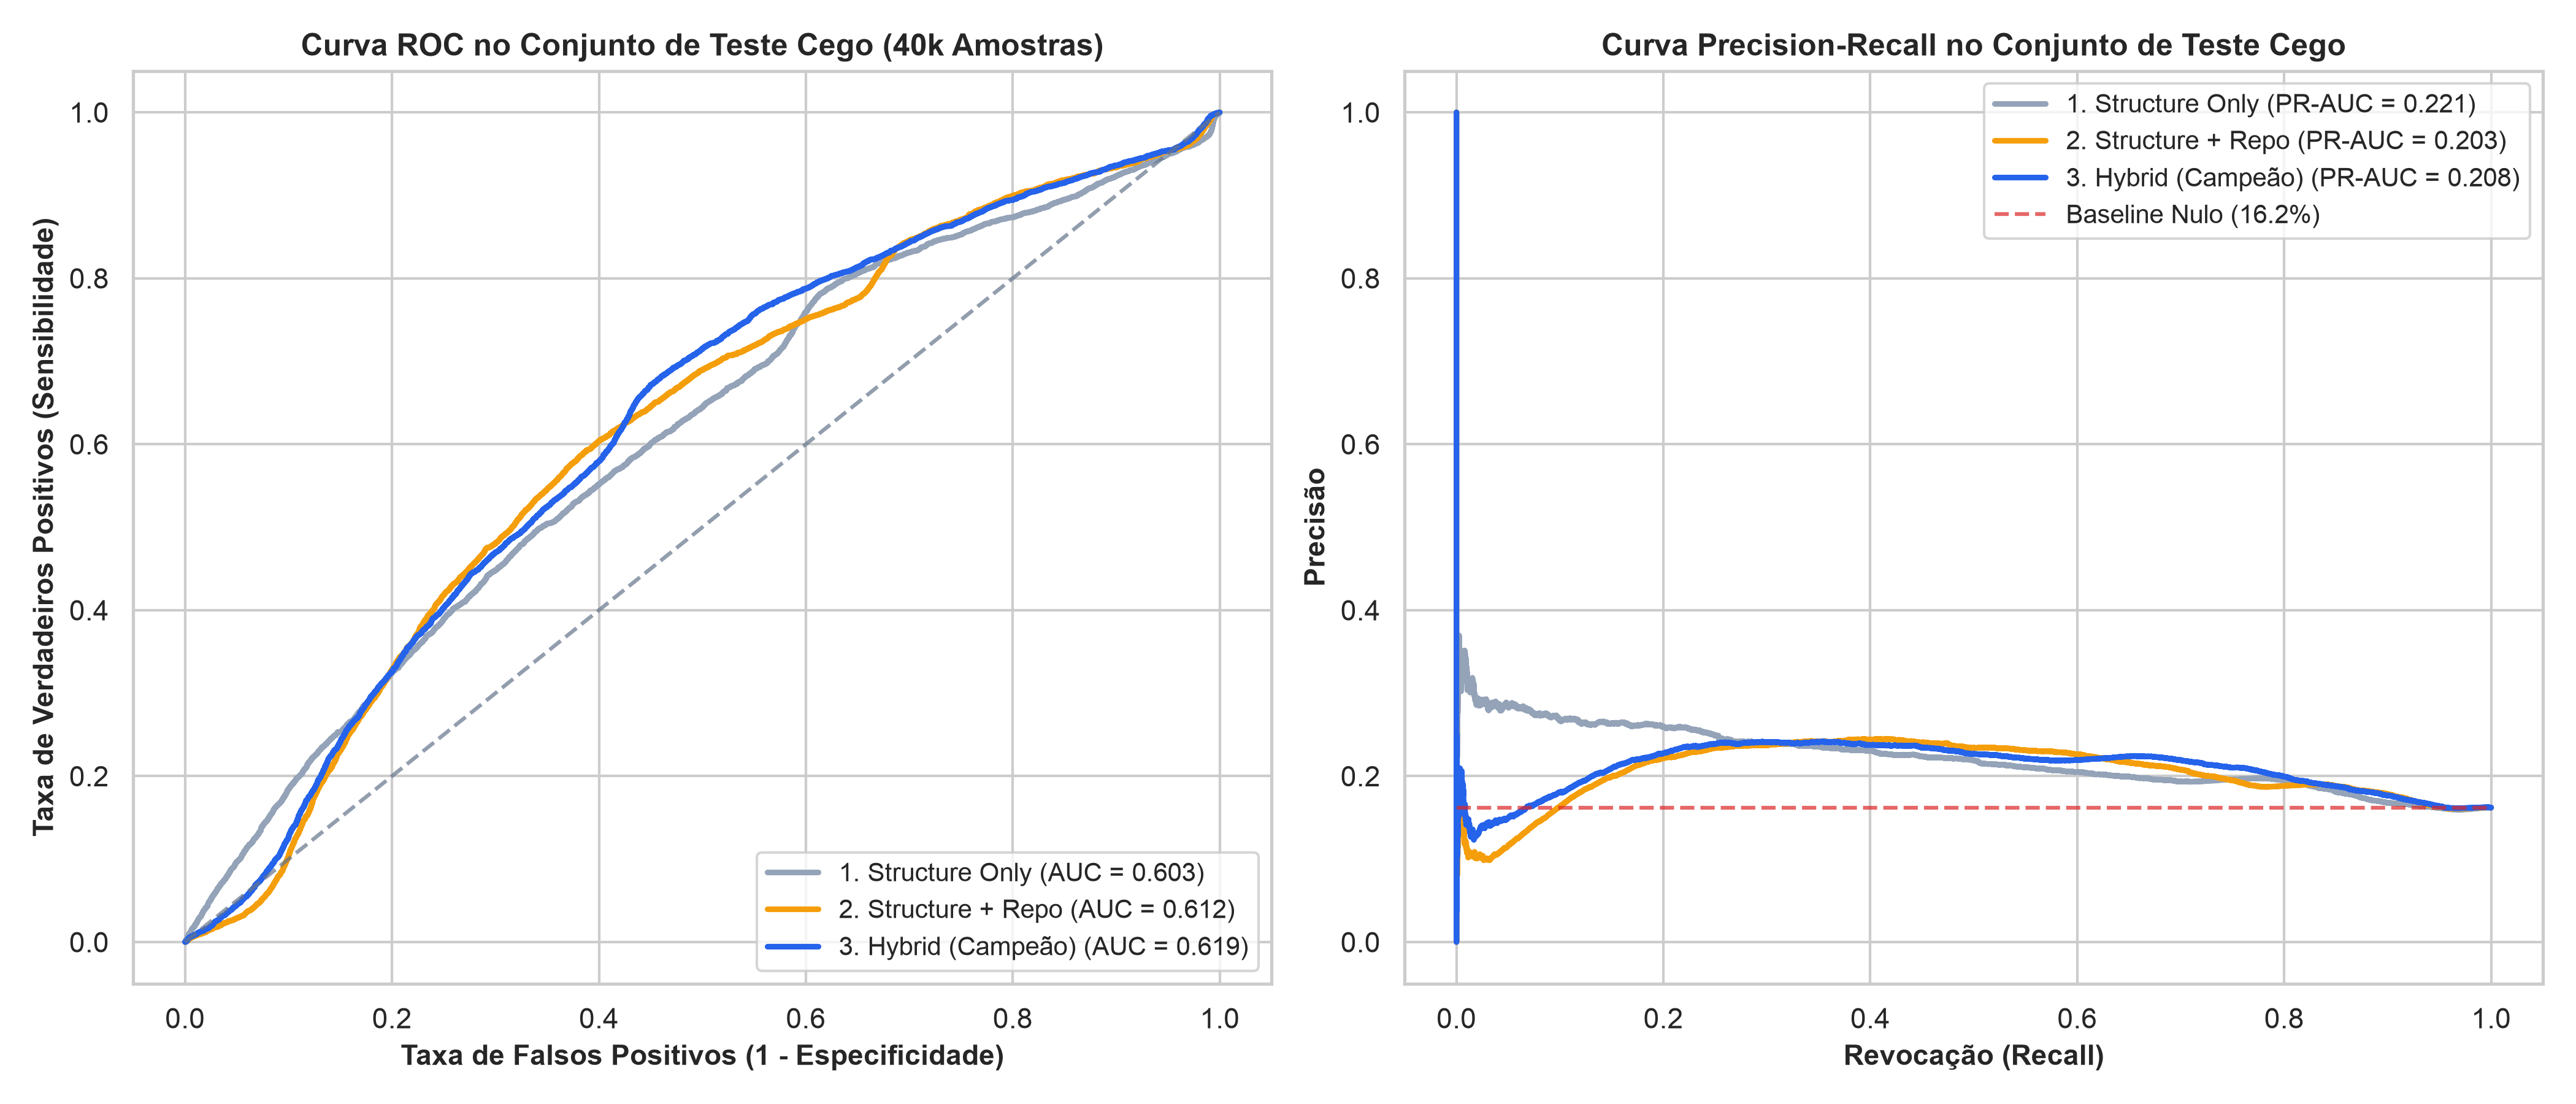
\includegraphics[width=\textwidth]{figures/final_test_roc_pr_curves.png}
        \caption{Blind test ROC and PR curves.}
    \end{subfigure}
    \hfill
    \begin{subfigure}[b]{0.48\columnwidth}
        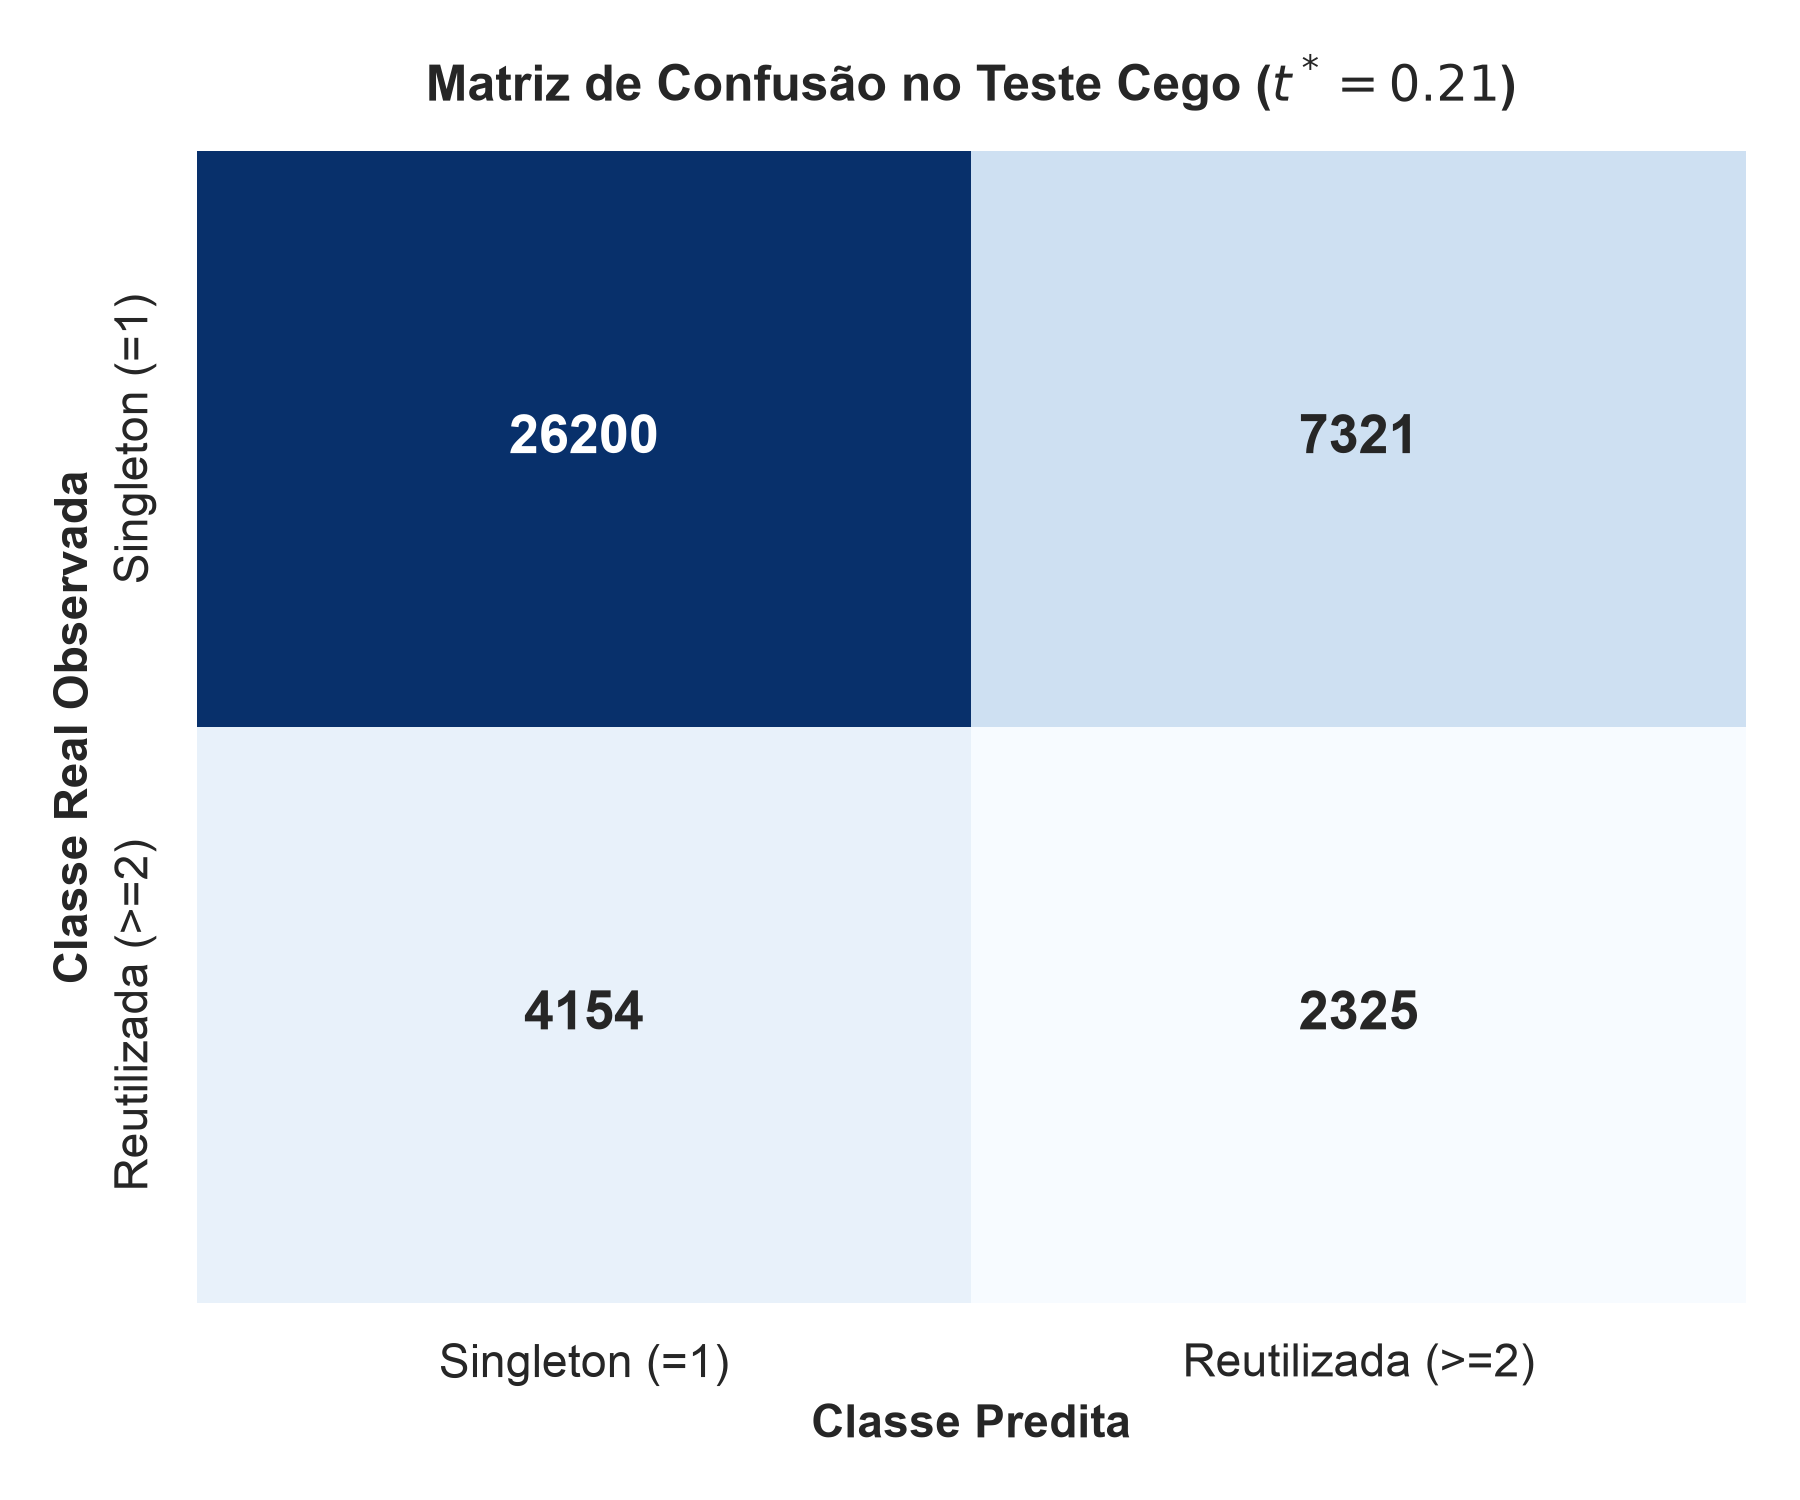
\includegraphics[width=\textwidth]{figures/final_test_confusion_matrix.png}
        \caption{Confusion matrix ($t^* = 0.21$).}
    \end{subfigure}
    \caption{Blind external evaluation on 40,000 instances from 14,568 foreign repos.}
    \label{fig:blind_test_plots}
\end{figure}

\subsection{Blind External Evaluation (40,000 Test Instances)}
Evaluating the frozen pipeline on 40,000 instances from 14,568 unseen repositories (Table~\ref{tab:blind_test}, Fig.~\ref{fig:blind_test_plots}) confirms our findings:
\begin{itemize}
    \item \textbf{Generalization Stability}: In cross-validation, the hybrid model scored $0.6706 \pm 0.0633$. On 14,568 untouched external repositories, it achieved $\mathbf{0.6211}$ ROC-AUC, falling within the 1-standard-deviation window ($[0.6073, 0.7339]$).
    \item \textbf{Threshold Impact}: The frozen threshold ($t^* = 0.21$) elevated test $F_1$ from $0.0727$ to $\mathbf{0.2967}$, recovering \textbf{2,376 true positive reused skills} with $78.16\%$ specificity ($26,200$ true negatives).
    \item \textbf{Viral Recovery}: On conditional intensity, the model achieved Class 3 Recall of $\mathbf{49.52\%}$ ($F_1 = 0.3163$). The classifier successfully flags half of all massively diffused skills in completely foreign repositories.
\end{itemize}

\section{Implications for Practice and Tooling}
Our findings offer concrete guidelines for agent skill creators:
\begin{enumerate}
    \item \textbf{Standardize File Locations}: Place skills at \texttt{.gemini/antigravity/skills/<skill>/SKILL.md} or \texttt{.agent/skills/}. Avoid non-standard naming.
    \item \textbf{Enforce Frontmatter Schemas}: Always provide valid delimited YAML declaring \texttt{name} and \texttt{description}.
    \item \textbf{Structure Contractual Prompt Headers}: Incorporate explicit markdown sections for \texttt{\#\# Objective}, \texttt{\#\# Role}, \texttt{\#\# Rules \& Constraints}, and \texttt{\#\# Examples}.
    \item \textbf{Specify Negative Boundaries}: Explicitly declare \texttt{\#\# Limitations} to restrict erroneous agent tool invocation.
\end{enumerate}

\section{Ethical Implications}
In accordance with challenge requirements, we consider the ethical dimensions of mining and modeling agent skills:
\begin{itemize}
    \item \textbf{Privacy and Anonymization}: We analyze public GitHub repositories without collecting or predicting personally identifiable information (PII). Developer accounts were anonymized in GitSkills commit tables, and our models operate exclusively on content hashes and repository-level aggregates.
    \item \textbf{Prompt Intellectual Property}: Decentralized skill copying without a registry risks obscuring original attribution. Our study emphasizes that transparent license and frontmatter declarations foster ethical attribution in agent ecosystems.
    \item \textbf{Supply-Chain Security}: Unverified skill propagation introduces vulnerability vectors (e.g., executing arbitrary shell commands). Understanding reuse patterns enables future automated security scanners to audit widely copied skills.
    \item \textbf{Computational Sustainability (Green AI)}: By demonstrating that regularized linear models with sparse caching outperform heavy deep neural networks, our replication pipeline executes in under 2 minutes, minimizing computational carbon footprint.
\end{itemize}

\section{Conclusion}
This paper presented an empirical study predicting the cross-repository reuse and diffusion of AI agent skills in the GitSkills dataset. We unmasked shortcut learning in tree ensembles, proved the stability of regularized linear models with supervised $\chi^2$ screening, and uncovered the Three Pillars of Skill Reuse. By providing verified models, operational thresholds, and authoring guidelines, this work establishes empirical foundations for the engineering of reusable agent skills.

\section*{Replication and Open Science}
The complete replication package, sparse matrices, scripts, and an interactive 1-click Google Colab notebook are available anonymously at: \url{https://anonymous.4open.science/r/skillreuse-anon}.

\bibliographystyle{IEEEtran}
\bibliography{references}

\end{document}
